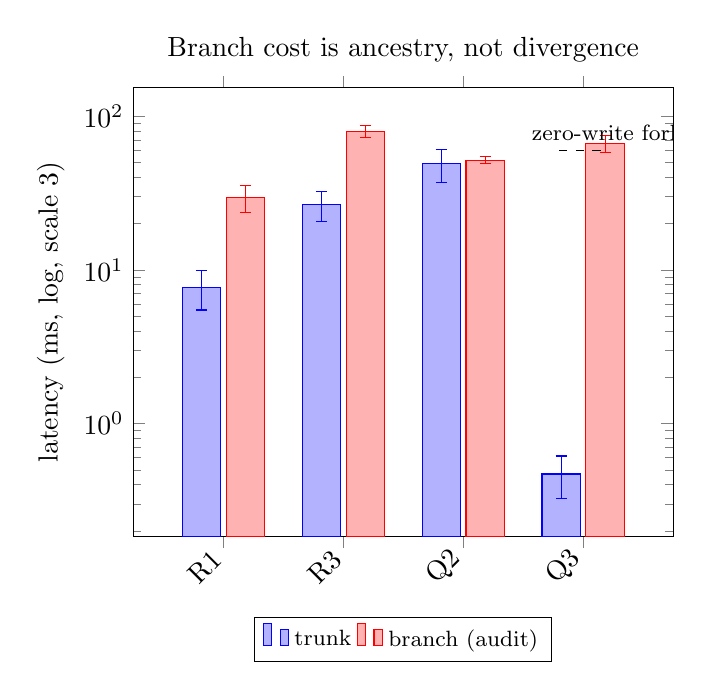
\begin{tikzpicture}
\begin{axis}[
  title={Branch cost is ancestry, not divergence},
  ylabel={latency (ms, log, scale 3)},
  ybar, bar width=0.32,
  enlarge x limits=0.25,
  ymode=log, log origin=infty,
  xtick=data,
  x tick label style={rotate=45,anchor=east},
  xticklabels={{R1},{R3},{Q2},{Q3}},
  legend style={at={(0.5,-0.18)},anchor=north,legend columns=-1,font=\footnotesize},
  error bars/y dir=both, error bars/y explicit,
]
  \addplot+[error bars/.cd,y explicit] coordinates {
    (1,7.688 ) +- (0.057,2.204 )
    (2,26.468 ) +- (5.767,5.827 )
    (3,49.019 ) +- (10.345,11.861 )
    (4,0.47 ) +- (0.01,0.146 )
  };
  \addlegendentry{trunk}
  \addplot+[error bars/.cd,y explicit] coordinates {
    (1,29.555 ) +- (5.446,5.972 )
    (2,79.782 ) +- (2.534,7.44 )
    (3,51.73 ) +- (7.94,2.604 )
    (4,66.205 ) +- (9.231,8.232 )
  };
  \addlegendentry{branch (audit)}
  \draw[dashed] (axis cs:3.8,59.627) -- (axis cs:4.2,59.627) node[above,font=\footnotesize] {zero-write fork};
\end{axis}
\end{tikzpicture}
{\footnotesize PRELIMINARY — non-reference hardware; medians of 5, bars show min/max. First readings, not reference figures (paper §5).\par}
